% Define document class
\documentclass[twocolumn]{aastex631}
\usepackage{showyourwork}
\usepackage{multirow}

% Glossaries
\usepackage[acronym,toc]{glossaries}
\newcommand*\myglsentry[1]{%
  \ifglsused{#1}{%
    \glsentryshort{#1}%
  }{%
    \glsentrylong{#1}%
  }%
}
\newacronym{scc}{SCC}{squamous cell carcinoma}
\newacronym{hnscc}{HNSCC}{head and neck \myglsentry{scc}}
\newacronym{opscc}{OPSCC}{oropharyngeal \myglsentry{scc}}
\newacronym{ctv}{CTV}{clinical target volume}
\newacronym{ctv-n}{CTV-N}{elective \myglsentry{ctv}}
\newacronym{lnl}{LNL}{lymph node level}
\newacronym{hmm}{HMM}{hidden Markov model}
\newacronym{rv}{RV}{random variable}
\newacronym{dag}{DAG}{directed acyclic graph}
\newacronym{mcmc}{MCMC}{Markov chain Monte Carlo}
\newacronym{ti}{TI}{thermodynamic integration}
\newacronym{bic}{BIC}{Bayesian information criterion}
\newacronym{bn}{BN}{Bayesian network}
\newacronym{ct}{CT}{computed tomography}
\newacronym{mri}{MRI}{magnetic resonance imaging}
\newacronym{pet}{PET}{positron emission tomography}
\newacronym{fna}{FNA}{fine needle aspiration}

% Cross-referencing
\usepackage{hyperref}
\AtEndPreamble{\usepackage{cleveref}}

% Begin!
\begin{document}

% Title
\title{Modelling the Lymphatic Metastatic Progression Pathways of OPSCC from Multi-Institutional Datasets}

% Author list
\author{Roman Ludwig}
\author{Jean-Marc Hoffmann}
\author{Bertrand Pouymayou}
\author{Panagiotis Balermpas}
\author{Lauence Bauwens}
\author{Vincent Grégoire}
\author{Roland Giger}
\author{Jan Unkelbach}

% Abstract
\begin{abstract}
    The \gls{ctv-n}\glsunset{ctv} definition in \gls{hnscc}\glsunset{scc} is currently based mostly on the prevalence of lymphatic metastases in different \glspl{lnl} based on the primary tumor location. In this work, we present an extension to a probabilistic model for lymphatic metastatic spread developed earlier that can quantify the risk for microscopic nodal involvement based on individual diagnoses. The extension is based on the same formalism of \glspl{hmm} as the original model, but in addition to the \glspl{lnl} I, II, III, and IV, it also covers the \glspl{lnl} V and VII of the ipsilateral neck. Moreover, we infer which pathways of lymphatic spread to model from clinical lymphatic progression patterns of 681 patients from three institutions. The extended model may allow for a more personalized \gls{ctv-n} definition based on a patient's individual state of disease. The \gls{hmm} uses a collection of hidden binary \glspl{rv} -- one for each \gls{lnl} -- to model a patient's state of lymphatic involvement. Clinical diagnoses and/or pathological examinations of resected \glspl{lnl} represent the observed binary \glspl{rv} corresponding to the unobservable true state of nodal disease. A \gls{dag} with parametrized edges is used to compute the transition matrix of the \gls{hmm} and consequently the (log-)likelihood of the diagnoses of 681 patients, given a set of spread parameters. Based on the defined likelihood function, \gls{mcmc} sampling is then used to infer a distribution over the model's parameters. T-category is model by assuming that, on average, patients with late T-category tumors are diagnosed at a later time compared to patients with early T-category tumors. Using \gls{ti} and the \gls{bic} we compare models based on different \glspl{dag} and demonstrate the accuracy and precision of the best-performing model. When extended to the contralateral side, this model may form the basis of future guidelines of elective \gls{ctv} definition.
\end{abstract}

% Main body
\section{Introduction}
\label{sec:intro}

When treating \gls{hnscc}, either with radiotherapy or via surgery, the aim is to irradiate or resect as much of the present malignancies as possible. This includes the primary tumor mass and metastases that are sufficiently large to be detected using in-vivo imaging modalities such as \gls{ct}, \gls{mri}, or \gls{pet}. But it also includes regions of possible microscopic spread, which these modalities cannot detect, to increase the patient's probability of cure \cite{poortmans_internal_2020,murthy_prostate-only_2021}. Microscopic disease can currently only be observed by a pathological examination of the tissue. Consequently, clinicians that are presented with cancer patients need to routinely assess the risk of microscopic involvement in parts of the body that appear clinically node negative.

This work concerns itself with \gls{opscc}, which commonly spreads lymphatically. The only two publicly available datasets on nodal involvement patterns in \gls{opscc}, at the time of writing, show that 80\% of patients where either cN+ or -- if available -- pN+ \cite{ludwig_dataset_2022}. Since the exact number and location of lymph nodes varies from patient to patient, the nodes are grouped into anatomically defined \glspl{lnl}. These levels are then often irradiated or resected prophylactically due to the risk of harboring occult metastases despite negative findings from imaging modalities. In current clinical practice, \gls{ctv-n} definition is instead mostly based on guidelines \cite{gregoire_ct-based_2003,gregoire_delineation_2014,gregoire_delineation_2018,eisbruch_intensity-modulated_2002,biau_selection_2019,chao_determination_2002,vorwerk_guidelines_2011,ferlito_elective_2009} that are derived from the observed prevalence of involvement in an \gls{lnl} for a given tumor location.

These guidelines, however, do not account for the personal risk of the patients that may depend greatly on their diagnosis. E.g., macroscopic metastases detected via \gls{pet} in the \glspl{lnl} II and III may increase the risk for occult disease in \gls{lnl} IV over the case of a patient who presents with a clinically N0 neck.

A model for estimating the risk of microscopic disease, given a personal diagnosis based on \glspl{bn} was previously developed \cite{pouymayou_bayesian_2019} and subsequently adapted to make use of \glspl{hmm} to include T-category in an intuitive manner \cite{ludwig_hidden_2021}. These models were trained on a dataset of early T-category (T1 and T2) patients that could be reconstructed from \cite{sanguineti_defining_2009}. Since this publication only includes details about the involvement of the ipsilateral \glspl{lnl} I, II, III, and IV, the models were limited to these nodal levels as well.

With the publication of larger and more detailed datasets \cite{ludwig_dataset_2022}, the risk estimation models may be extended as well to include the additionally reported \glspl{lnl} V and VII. This work aims to do that and at the same time demonstrate the capability 
of the previously introduced \gls{hmm} to adapt to real patient data from a multi-centric cohort of XXX \gls{opscc} patients.

\section{Previous Work}
\label{sec:previous_work}

\subsection{Lymphatic Spread as Hidden Markov Model}
\label{subsec:previous_work:spread_as_hmm}

We have introduced a probabilistic model for lymphatic metastatic tumor progression based on \glspl{bn} in \cite{pouymayou_bayesian_2019} and based off of this an improved model using \glspl{hmm} in \cite{ludwig_hidden_2021}. We will briefly recap the \acrlong{hmm} below.

A patient's state of (hidden) lymphatic involvement at time $t$ is described as a collection of binary \glspl{rv}, one for each of the $V$ \glspl{lnl}:
%
\begin{equation}
    \mathbf{X}[t] = \left( X_v[t] \right) \qquad v \in \left\{ 1,2, \ldots, V \right\}
\end{equation}
%
Where each of the \glspl{lnl} can be in the state $X_v=0$ (\texttt{FALSE}), meaning \gls{lnl} $v$ is healthy, or in the state $X_v=1$ (\texttt{TRUE}), indicating the \gls{lnl} harbors metastases.

The transition from one time-step to another is governed by the transition probability $P\left( \mathbf{X}[t+1]=\boldsymbol{\xi}_i \mid \mathbf{X}[t]=\boldsymbol{\xi}_j \right)$, which can conveniently be collected into a transition matrix when we enumerate all $2^V$ distinct possible states $\boldsymbol{\xi}_i$ with $i \in \left\{ 1,2, \ldots, 2^V \right\}$ of lymphatic involvement:
%
\begin{equation}
    \mathbf{A} = \left( A_{ij} \right) = \left( P\left( \mathbf{X}[t+1]=\boldsymbol{\xi}_i \mid \mathbf{X}[t]=\boldsymbol{\xi}_j \right) \right)
\end{equation}
%
The term $P\left( \boldsymbol{\xi}_i \mid \boldsymbol{\xi}_j \right)$ describes the probability to transition from the hidden state of lymphatic involvement $\boldsymbol{\xi}_j$ to the state $\boldsymbol{\xi}_i$ within between the time $t$ and $t+1$. Using a \gls{dag} as depicted in \cref{fig:graph_with_obs}, we can parameterize this transition probability in the following way:
%
\begin{equation}
    \label{eq:transition_prob}
    P\left( \boldsymbol{\xi}_i \mid \boldsymbol{\xi}_j \right) = \prod_{v \leq V} Q\left( \xi_{iv} ; \xi_{jv} \right) P \left( \xi_{iv} \mid \left\{ \xi_{jr} \right\}_{r \in \operatorname{pa}(v)} \right)^{1 - \xi_{jv}}
\end{equation}
%
In this equation, we have denoted \glspl{lnl} that are parents of \gls{lnl} $v$ with the symbol $r\in\operatorname{pa}(v)$. Also, $\xi_{iv}$ denotes the value that \gls{lnl} $v$ takes on when the patient is in state $\boldsymbol{\xi}_i$. Lastly, the term $Q(a;b) \in \{ 0,1 \}$ is there only to 

\begin{figure}
    \centering
    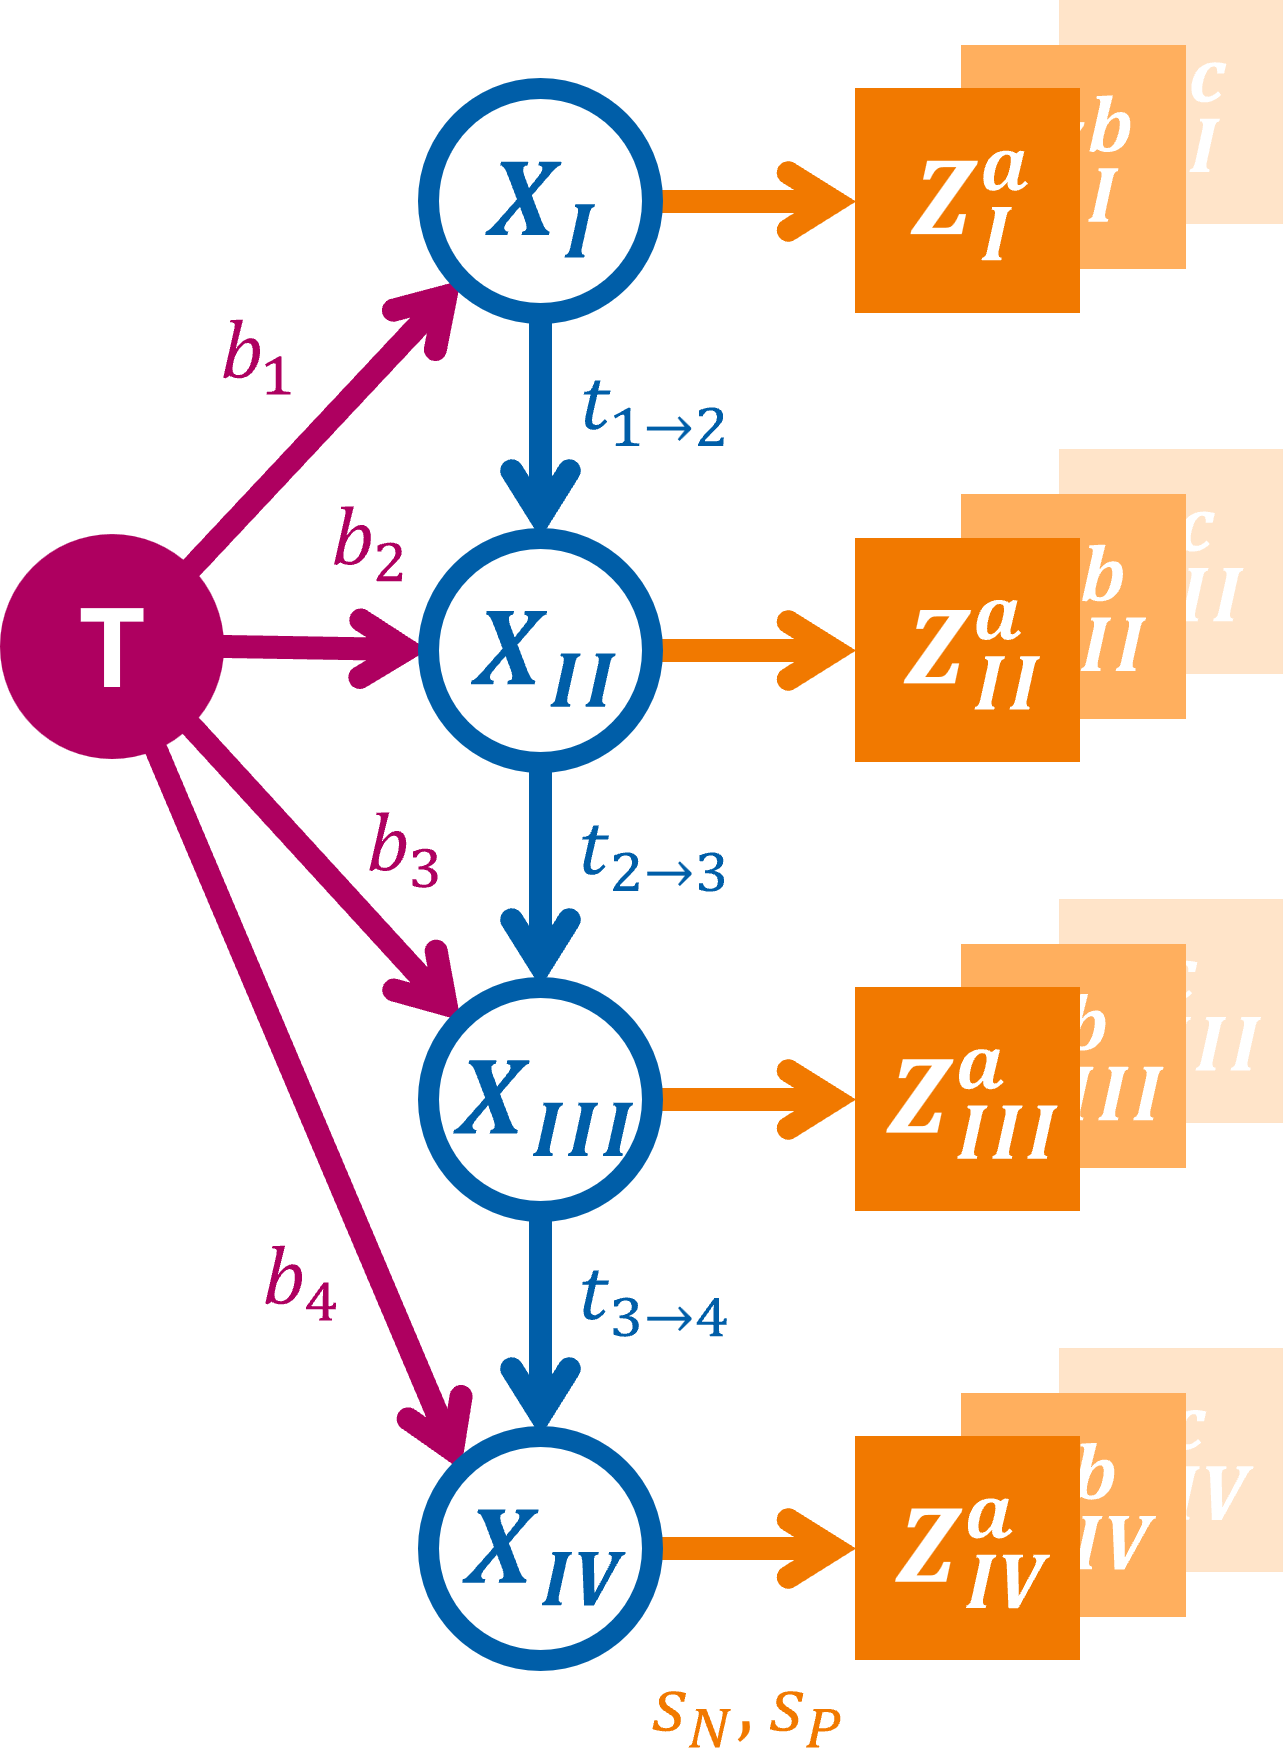
\includegraphics[width=0.6\linewidth]{figures/graph_with_obs.png}
    \caption{\Gls{dag} representing a possible abstraction of the lymphatic network comprising the tumor (red shaded circle) and \glspl{lnl} I through IV as hidden binary \glspl{rv} (blue outlined circles). Attached to each of these is the corresponding observed \gls{rv} (orange shaded squares). Lymphatic flow is depicted in the form of parameterized arrows (red and blue) that represent the probability of spread along the respective arc per time-step. Sensitivity and specificity (orange arrows) connect the hidden \glspl{rv} to the diagnosis.}
    \label{fig:graph_with_obs}
\end{figure}

Diagnosis and true state of a patient are formally connected via the sensitivity $s_N$ and specificity $s_P$ of the used diagnostic modality. In clinical practice, these modalities are \gls{ct}, \gls{mri}, or \gls{pet} scan, but it may also include information from biopsies after a \gls{fna} or other techniques to detect lymphatic metastases. For each \gls{lnl} $v$ the conditional probability table of $P\left( Z_v \mid X_v \right)$ looks like this:

\noindent
\begin{center}
    \begin{tabular}{|cc|cc|}
        \hline
        & & \multicolumn{2}{c|}{$X$} \\
        & & 0 & 1 \\
        \hline
        \multirow{2}{*}{$Z$} & 0 & $s_p$ & $1 - s_N$ \\
        & 1 & $1 - s_P$ & $s_N$ \\
        \hline
    \end{tabular}
\end{center}

Consequently, the conditional probability to observe a diagnosis $\mathbf{Z}=\boldsymbol{\zeta}_\ell$, given a hidden involvement state $\mathbf{X}=\boldsymbol{\xi}_k$ is a matrix $\mathbf{B}$ made up of products of terms from the table above:
%
\begin{equation} \label{eq:transition_matrix}
    \mathbf{B} = \left( B_{k\ell} \right) = \prod_{v=1}^V P\left( Z_v = \zeta_{\ell v} \mid X_v[t_\text{D}] = \xi_{kv} \right)
\end{equation}

If multiple diagnostic modalities $\mathcal{O} \in \{ \text{MRI}, \text{CT}, \ldots \}$ are used, one can compute an observation matrix $\mathbf{B}^\mathcal{O}$ for each of these modalities and combine them via an outer product into a joint observations matrix:
%
\begin{equation}
    \mathbf{B} = \mathbf{B}^\text{MRI} \otimes \mathbf{B}^\text{CT} \otimes \ldots
\end{equation}

We define the time $t=0$ to be the moment just before a patient's tumor formed, and hence $X_v[t=0]=0 \,\,\, \forall v$. However, using this definition, we cannot know how many time-steps have passed until $t_\text{D}$, when the patient was diagnosed with cancer. We can only make the assumption that a patients with an earlier T-category tumor was \emph{probably} diagnosed after fewer time-steps than a patient with a late T-category tumor. We can use this information by marginalizing over the diagnose times $t_\text{D}$ of patients in different T-categories using different prior distributions over the diagnose time. E.g., $P \left( t=t_D \mid \text{early} \right)$ for early T-category patients (T1 \& T2) and $P \left( t=t_D \mid \text{late} \right)$ for late T-category patients (T3 \& T4). Throughout this work we will use binomial distributions for these probability mass functions, mainly because they have a plausible shape for this purpose and only a single parameter.
%
\begin{equation}
    P \left( t = t_D \mid \text{T-cat.} \right) = \operatorname{B}(t_\text{max},p_\text{T-cat.})
\end{equation}
%
Here, the parameter $p_\text{early}$ can be interpreted as the probability that the patient will be diagnosed at time-step $t+1$ given they are in time-step $t$. We will use as a latest time-step $t_\text{max} = 10$.

\subsection{The Likelihood Function}
\label{subsec:previous_work:likelihood}

Using the definitions up to this point, we can compute a vector of likelihoods for every possible diagnosis:
%
\begin{equation} \label{eq:likelihood_vec}
\begin{split}
    \boldsymbol{\ell} &= \big( P\left( \mathbf{Z} = \boldsymbol{\zeta}_i \right) \big) \\
    &= \sum_{t=0}^{t_{max}} \left[ \boldsymbol{\pi} \cdot \mathbf{A}^t \cdot \mathbf{B} \right] \cdot P \left( t \mid \text{T-cat.} \right)
\end{split}
\end{equation}
%
This likelihood implicitly depends on how we parameterize the arcs of the \gls{dag} underlying the model and the parameterization of the distribution over diagnosis times. If we use the graph displayed in \cref{fig:graph_with_obs}, we can write down a conditional probability table for \gls{lnl} $X_3$ being healthy or metastatic, based on the state of the parent \gls{lnl} $\operatorname{pa}(3) = 2$:

\noindent
\begin{center}
    \begin{tabular}{|cc|cc|}
        \hline
        & & \multicolumn{2}{c|}{$X_2$} \\
        & & 0 & 1 \\
        \hline
        \multirow{2}{*}{$X_3$} & 0 & $1 - b_3$ & $(1 - b_3)(1 - t_{23})$ \\
        & 1 & $b_3$ & $1 - b_3 - t_{23} + b_3 t_{23}$ \\
        \hline
    \end{tabular}
\end{center}

Similar tables can be written for all other \glspl{lnl}. The terms in these conditional probability tables can then be used to compute the transition probability between to particular states $\boldsymbol{\xi}_i$ and $\boldsymbol{\xi}_j$ as in \cref{eq:transition_prob}. Computing this quantity for all possible transitions subsequently yields the transition matrix $\mathbf{A}$ as described in \cref{eq:transition_matrix}.

Together with the parametrizations of the distributions over the diagnosis time, the parameters that make up the transition matrix $\mathbf{A}$ comprises the set of model parameters:
%
\begin{equation}
    \boldsymbol{\theta} = \left( \left\{ b_v \right\}, \left\{ t_{vr} \right\}, p_\text{early}, p_\text{late} \right) \quad \text{with} \quad \genfrac{}{}{0pt}{2}{v\leq V}{r\in\operatorname{pa}(v)}
\end{equation}

To infer these parameters from a dataset of $N$ \gls{hnscc} patients $\boldsymbol{\mathcal{D}} = \left( d_1, d_2, \ldots, d_N \right)$, we compute the data log-likelihood:
%
\begin{equation}
    \log\mathcal{L} \left( \boldsymbol{\mathcal{D}} \mid \boldsymbol{\theta} \right) = \sum_{i=1}^N \log P \left( \mathbf{Z} = d_i \right)
\end{equation}
%
Which effectively amounts to computing the element-wise logarithm of the likelihood vector $\boldsymbol{\ell}$ from \cref{eq:likelihood_vec} and summing up the entries that correspond to each of the patients $d_i$ for $i\leq N$. 

Using this log-likelihood function one may now employ a variety of inference methods to learn the parameters of the model that best describe the observed data. After that, the main task of of personalizing the \gls{ctv-n} definition is to predict the probability of the hidden possible states $\boldsymbol{\xi}_k$ given the diagnosis $d^\star=\boldsymbol{\zeta}_\ell$ of a new patient. Using Bayes' theorem, we get
%
\begin{equation}
    P\left( \mathbf{X}=\boldsymbol{\xi}_k \mid \mathbf{Z}=\boldsymbol{\zeta}_\ell \right) = \frac{P\left( \boldsymbol{\zeta}_\ell \mid \boldsymbol{\xi}_k \right) P\left( \boldsymbol{\xi}_k \mid \boldsymbol{\theta} \right)}{\sum_{r=1}^{2^V} P\left( \boldsymbol{\zeta}_\ell \mid \boldsymbol{\xi}_r \right) P\left( \boldsymbol{\xi}_r \mid \boldsymbol{\theta} \right) }
\end{equation}
%
The described model along with the inferred parameters $\boldsymbol{\hat{\theta}}$ will yield an estimate (or multiple estimates) for the ``prior'' in the above equation $P\big( \boldsymbol{\xi}_k \mid \boldsymbol{\hat{\theta}} \big)$.

\begin{figure*}
    \script{bg_core_prevs.py}
    \begin{centering}
        \includegraphics[width=\textwidth]{figures/bg_core_prevs.png}
        \caption{Testing this showyourwork thingy}
        \label{fig:bg_prevalences}
    \end{centering}
\end{figure*}

\begin{figure}
    \script{comp_IandII_low_prevs.py}
    \begin{centering}
        \includegraphics[width=\linewidth]{figures/comp_IandII_low_prevs.png}
        \caption{This should be a one-column wide figure.}
        \label{fig:IandII_low_prevs}
    \end{centering}
\end{figure}

\begin{figure}
    \script{comp_IandII_high_prevs.py}
    \begin{centering}
        \includegraphics[width=\linewidth]{figures/comp_IandII_high_prevs.png}
        \caption{This should be a one-column wide figure.}
        \label{fig:IandII_high_prevs}
    \end{centering}
\end{figure}

\bibliography{bib}

\end{document}
